% !TEX program = xelatex
\documentclass[a4paper,14pt,oneside,openany]{memoir}

%%% Задаем поля, отступы и межстрочный интервал %%%
\usepackage{amsmath}
\usepackage[left=30mm, right=15mm, top=20mm, bottom=20mm]{geometry} % Пакет geometry с аргументами для определения полей
\pagestyle{plain} % Убираем стандарные для данного класса верхние колонтитулы с заголовком текущей главы, оставляем только номер страницы снизу по центру
\parindent=1.25cm % Абзацный отступ 1.25 см, приблизительно равно пяти знакам, как по ГОСТ
\usepackage{indentfirst} % Добавляем отступ к первому абзацу
%\linespread{1.3} % Межстрочный интервал (наиболее близко к вордовскому полуторному) - тут вместо этого используется команда OnehalfSpacing*

%%% Задаем языковые параметры и шрифт %%%

\usepackage[english, russian]{babel}                % Настройки для русского языка как основного в тексте
\babelfont{rm}{Times New Roman}                     % TMR в качестве базового roman-щрифта

%%% Задаем стиль заголовков и подзаголовков в тексте %%%

\setsecnumdepth{subsection} % Номера разделов считать до третьего уровня включительно, т.е. нумеруются только главы, секции, подсекции
\renewcommand*\chapterheadstart{} % Переопределяем команду, задающую отступ над заголовком, чтобы отступа не было
\renewcommand*\printchaptername{} % Переопределяем команду, печатающую слово "Глава", чтобы оно не печалось
%\renewcommand*\printchapternum{} % То же самое для номера главы - тут не надо, номер главы оставляем
\renewcommand*\chapnumfont{\normalfont\bfseries} % Меняем стиль шрифта для номера главы: нормальный размер, полужирный
\renewcommand*\afterchapternum{\hspace{1em}} % Меняем разделитель между номером главы и названием
\renewcommand*\printchaptertitle{\normalfont\bfseries\centering\MakeUppercase} % Меняем стиль написания для заголовка главы: нормальный размер, полужирный, центрированный, заглавными буквами
\setbeforesecskip{20pt} % Задаем отступ перед заголовком секции
\setaftersecskip{20pt} % Ставим такой же отступ после заголовка секции
\setsecheadstyle{\raggedright\normalfont\bfseries} % Меняем стиль написания для заголовка секции: выравнивание по правому краю без переносов, нормальный размер, полужирный
\setbeforesubsecskip{20pt} % Задаем отступ перед заголовком подсекции
\setaftersubsecskip{20pt} % Ставим такой же отступ после заголовка подсекции
\setsubsecheadstyle{\raggedright\normalfont\bfseries}  % Меняем стиль написания для заголовка подсекции: выравнивание по правому краю без переносов, нормальный размер, полужирный

%%% Задаем параметры оглавления %%%

\addto\captionsrussian{\renewcommand\contentsname{Содержание}} % Меняем слово "Оглавление" на "Содержание"
\setrmarg{2.55em plus1fil} % Запрещаем переносы слов в оглавлении
%\setlength{\cftbeforechapterskip}{0pt} % Эта команда убирает интервал между заголовками глав - тут не надо, так красивее смотрится
\renewcommand{\aftertoctitle}{\afterchaptertitle \vspace{-\cftbeforechapterskip}} % Делаем отступ между словом "Содержание" и первой строкой таким же, как у заголовков глав
%\renewcommand*\chapternumberline[1]{} % Делаем так, чтобы номер главы не печатался - тут не надо
\renewcommand*\cftchapternumwidth{1.5em} % Ставим подходящий по размеру разделитель между номером главы и самим заголовком
\renewcommand*\cftchapterfont{\normalfont\MakeUppercase} % Названия глав обычным шрифтом заглавными буквами
\renewcommand*\cftchapterpagefont{\normalfont} % Номера страниц обычным шрифтом
\renewcommand*\cftchapterdotsep{\cftdotsep} % Делаем точки до номера страницы после названий глав
\renewcommand*\cftdotsep{1} % Задаем расстояние между точками
\renewcommand*\cftchapterleader{\cftdotfill{\cftchapterdotsep}} % Делаем точки стандартной формы (по умолчанию они "жирные")
\maxtocdepth{subsection} % В оглавление попадают только разделы первыхтрех уровней: главы, секции и подсекции

%%% Выравнивание и переносы %%%

%% http://tex.stackexchange.com/questions/241343/what-is-the-meaning-of-fussy-sloppy-emergencystretch-tolerance-hbadness
%% http://www.latex-community.org/forum/viewtopic.php?p=70342#p70342
\tolerance 1414
\hbadness 1414
\emergencystretch 1.5em                             % В случае проблем регулировать в первую очередь
\hfuzz 0.3pt
\vfuzz \hfuzz
%\dbottom
%\sloppy                                            % Избавляемся от переполнений
\clubpenalty=10000                                  % Запрещаем разрыв страницы после первой строки абзаца
\widowpenalty=10000                                 % Запрещаем разрыв страницы после последней строки абзаца
\brokenpenalty=4991                                 % Ограничение на разрыв страницы, если строка заканчивается переносом

%%% Объясняем компилятору, какие буквы русского алфавита можно использовать в перечислениях (подрисунках и нумерованных списках) %%%
%%% По ГОСТ нельзя использовать буквы ё, з, й, о, ч, ь, ы, ъ %%%
%%% Здесь также переопределены заглавные буквы, хотя в принципе они в документе не используются %%%

\makeatletter
    \def\russian@Alph#1{\ifcase#1\or
       А\or Б\or В\or Г\or Д\or Е\or Ж\or
       И\or К\or Л\or М\or Н\or
       П\or Р\or С\or Т\or У\or Ф\or Х\or
       Ц\or Ш\or Щ\or Э\or Ю\or Я\else\xpg@ill@value{#1}{russian@Alph}\fi}
    \def\russian@alph#1{\ifcase#1\or
       а\or б\or в\or г\or д\or е\or ж\or
       и\or к\or л\or м\or н\or
       п\or р\or с\or т\or у\or ф\or х\or
       ц\or ш\or щ\or э\or ю\or я\else\xpg@ill@value{#1}{russian@alph}\fi}
\makeatother

%%% Задаем параметры оформления рисунков и таблиц %%%

\usepackage{graphicx, caption, subcaption} % Подгружаем пакеты для работы с графикой и настройки подписей
\graphicspath{{images/}} % Определяем папку с рисунками
\captionsetup[figure]{font=small, width=\textwidth, name=Рисунок, justification=centering} % Задаем параметры подписей к рисункам: маленький шрифт (в данном случае 12pt), ширина равна ширине текста, полнотекстовая надпись "Рисунок", выравнивание по центру
\captionsetup[subfigure]{font=small} % Индексы подрисунков а), б) и так далее тоже шрифтом 12pt (по умолчанию делает еще меньше)
\captionsetup[table]{singlelinecheck=false,font=small,width=\textwidth,justification=justified} % Задаем параметры подписей к таблицам: запрещаем переносы, маленький шрифт (в данном случае 12pt), ширина равна ширине текста, выравнивание по ширине
\captiondelim{ --- } % Разделителем между номером рисунка/таблицы и текстом в подписи является длинное тире
\setkeys{Gin}{width=\textwidth} % По умолчанию размер всех добавляемых рисунков будет подгоняться под ширину текста
\renewcommand{\thesubfigure}{\asbuk{subfigure}} % Нумерация подрисунков строчными буквами кириллицы
%\setlength{\abovecaptionskip}{0pt} % Отбивка над подписью - тут не меняем
%\setlength{\belowcaptionskip}{0pt} % Отбивка под подписью - тут не меняем
\usepackage[section]{placeins} % Объекты типа float (рисунки/таблицы) не вылезают за границы секциии, в которой они объявлены
\usepackage{float} % Пакет для контроля размещения плавающих объектов

%%% Задаем параметры ссылок и гиперссылок %%%

\usepackage{hyperref}                               % Подгружаем нужный пакет
\hypersetup{
    colorlinks=true,                                % Все ссылки и гиперссылки цветные
    linktoc=all,                                    % В оглавлении ссылки подключатся для всех отображаемых уровней
    linktocpage=true,                               % Ссылка - только номер страницы, а не весь заголовок (так выглядит аккуратнее)
    linkcolor=red,                                  % Цвет ссылок и гиперссылок - красный
    citecolor=red                                   % Цвет цитировний - красный
}

%%% Настраиваем отображение списков %%%

\usepackage{enumitem}                               % Подгружаем пакет для гибкой настройки списков
\renewcommand*{\labelitemi}{\normalfont{--}}        % В ненумерованных списках для пунктов используем короткое тире
\makeatletter
    \AddEnumerateCounter{\asbuk}{\russian@alph}     % Объясняем пакету enumitem, как использовать asbuk
\makeatother
\renewcommand{\labelenumii}{\asbuk{enumii})}        % Кириллица для второго уровня нумерации
\renewcommand{\labelenumiii}{\arabic{enumiii})}     % Арабские цифры для третьего уровня нумерации
\setlist{noitemsep, leftmargin=*}                   % Убираем интервалы между пунками одного уровня в списке
\setlist[1]{labelindent=\parindent}                 % Отступ у пунктов списка равен абзацному отступу
\setlist[2]{leftmargin=\parindent}                  % Плюс еще один такой же отступ для следующего уровня
\setlist[3]{leftmargin=\parindent}                  % И еще один для третьего уровня

%%% Счетчики для нумерации объектов %%%

\counterwithout{figure}{chapter}                    % Сквозная нумерация рисунков по документу
\counterwithout{equation}{chapter}                  % Сквозная нумерация математических выражений по документу
\counterwithout{table}{chapter}                     % Сквозная нумерация таблиц по документу

%%% Реализация библиографии пакетами biblatex и biblatex-gost с использованием движка biber %%%

\usepackage{csquotes} % Пакет для оформления сложных блоков цитирования (biblatex рекомендует его подключать)
\usepackage[%
backend=biber,                                      % Движок
bibencoding=utf8,                                   % Кодировка bib-файла
sorting=none,                                       % Настройка сортировки списка литературы
style=gost-numeric,                                 % Стиль цитирования и библиографии по ГОСТ
language=auto,                                      % Язык для каждой библиографической записи задается отдельно
autolang=other,                                     % Поддержка многоязычной библиографии
sortcites=true,                                     % Если в квадратных скобках несколько ссылок, то отображаться будут отсортированно
movenames=false,                                    % Не перемещать имена, они всегда в начале библиографической записи
maxnames=5,                                         % Максимальное отображаемое число авторов
minnames=3,                                         % До скольки сокращать число авторов, если их больше максимума
doi=false,                                          % Не отображать ссылки на DOI
isbn=false,                                         % Не показывать ISBN, ISSN, ISRN
]{biblatex}[2016/09/17]
\DeclareDelimFormat{bibinitdelim}{}                 % Убираем пробел между инициалами (Иванов И.И. вместо Иванов И. И.)
\addbibresource{biba.bib}                           % Определяем файл с библиографией

%%% Скрипт, который автоматически подбирает язык (и, следовательно, формат) для каждой библиографической записи %%%
%%% Если в названии работы есть кириллица - меняем значение поля langid на russian %%%
%%% Все оставшиеся пустые места в поле langid заменяем на english %%%

\DeclareSourcemap{
  \maps[datatype=bibtex]{
    \map{
        \step[fieldsource=title, match=\regexp{^\P{Cyrillic}*\p{Cyrillic}.*}, final]
        \step[fieldset=langid, fieldvalue={russian}]
    }
    \map{
        \step[fieldset=langid, fieldvalue={english}]
    }
  }
}

%%% Прочие пакеты для расширения функционала %%%

\usepackage{longtable,ltcaption}                    % Длинные таблицы
\usepackage{multirow,makecell}                      % Улучшенное форматирование таблиц
\usepackage{booktabs}                               % Еще один пакет для красивых таблиц
\usepackage{soulutf8}                               % Поддержка переносоустойчивых подчёркиваний и зачёркиваний
\usepackage{icomma}                                 % Запятая в десятичных дробях
\usepackage{hyphenat}                               % Для красивых переносов
\usepackage{textcomp}                               % Поддержка "сложных" печатных символов типа значков иены, копирайта и т.д.
\usepackage[version=4]{mhchem}                      % Красивые химические уравнения
\usepackage{amsmath}                                % Усовершенствование отображения математических выражений 
\usepackage{amsfonts}
\usepackage{float}
%%% Вставляем по очереди все содержательные части документа %%%

\usepackage{listings}
\usepackage{color}
\definecolor{codegray}{rgb}{0.95,0.95,0.95}
\lstset{
  backgroundcolor=\color{codegray},
  basicstyle=\ttfamily\small,
  breaklines=true,
  frame=single,
  language=Python,
  showstringspaces=false
}

\begin{document}

\thispagestyle{empty}

\begin{center}
    МИНИСТЕРСТВО НАУКИ И ВЫСШЕГО ОБРАЗОВАНИЯ \\ РОССИЙСКОЙ ФЕДЕРАЦИИ

    \vspace{20pt}

    Федеральное государственное автономное \\ образовательное учреждение высшего образования \\
    "<Национальный исследовательский университет ИТМО"> \\
    (Университет ИТМО)

    \vspace{20pt}

    Факультет систем управления и робототехники

    \vspace{20pt}

    Дисциплина "Нелинейные системы управления"
\end{center}

\vfill

\begin{center}
    ОТЧЕТ \\
    по лабораторной работе №1

    \vspace{20pt}

    % по теме: \\
    % \uppercase{Singular Value Decomposition}
\end{center}

\vfill

    \noindent Студенты: \\
    \textit{Группа № R3435 \hfill Зыкин Л. В.} \\
    \textit{Группа № R3441 \hfill Алёхова М. С.} \\
    \textit{Группа № R3480 \hfill Кисиков Д. С.} \\

    \vspace{20pt}

    \noindent Предподаватель: \\
    \textit{доцент, ведущий научный сотрудник \hfill Зименко К. А.}

\vfill

\begin{center}
    Санкт-Петербург, 2025
\end{center}                                     % Титульник

\newpage % Переходим на новую страницу
\setcounter{page}{2} % Начинаем считать номера страниц со второй
\OnehalfSpacing* % Задаем полуторный интервал текста (в титульнике одинарный, поэтому команда стоит после него)

% \tableofcontents*                                   % Автособираемое оглавление

\section{Введение}

В данной лабораторной работе рассматриваются методы линеаризации обратной связью для нелинейных систем управления. Основное внимание уделяется анализу линеаризуемости по входу-выходу, преобразованию систем в нормальную форму и синтезу законов управления.

Основные задачи работы:
\begin{enumerate}
\item Анализ линеаризуемости по входу-выходу нелинейной системы
\item Преобразование системы в нормальную форму с указанием области определения
\item Проверка минимально-фазовости системы
\item Синтез закона управления методом линеаризации обратной связью для глобальной стабилизации
\end{enumerate}

Работа демонстрирует применение теоретических методов линеаризации обратной связью к практическим задачам управления нелинейными системами.

\section{Задача 1. Анализ линеаризуемости по входу-выходу}

Рассмотрим систему:
\begin{align}
\dot{x}_1 &= -x_1 + x_2 - x_3 \\
\dot{x}_2 &= -x_1 x_3 - x_2 + u \\
\dot{x}_3 &= -x_1 + u \\
y &= x_3
\end{align}

\subsection{Проверка линеаризуемости по входу-выходу}

Для проверки линеаризуемости по входу-выходу вычислим производные Ли выходной функции $h(x) = x_3$.

\textbf{Шаг 1:} Вычисление производных Ли
\begin{align}
L_f^0 h &= h = x_3 \\
L_f^1 h &= \frac{\partial h}{\partial x_1} f_1 + \frac{\partial h}{\partial x_2} f_2 + \frac{\partial h}{\partial x_3} f_3 \\
&= 0 \cdot (-x_1 + x_2 - x_3) + 0 \cdot (-x_1 x_3 - x_2) + 1 \cdot (-x_1 + u) \\
&= -x_1 + u
\end{align}

\textbf{Шаг 2:} Проверка условия линеаризуемости
\begin{align}
L_g L_f^0 h &= \frac{\partial h}{\partial x_1} g_1 + \frac{\partial h}{\partial x_2} g_2 + \frac{\partial h}{\partial x_3} g_3 \\
&= 0 \cdot 0 + 0 \cdot 1 + 1 \cdot 1 = 1 \neq 0
\end{align}

Поскольку $L_g L_f^0 h = 1 \neq 0$, система линеаризуема по входу-выходу с относительной степенью $r = 1$.

\subsection{Преобразование в нормальную форму}

Для системы размерности $n = 3$ с относительной степенью $r = 1$ размерность внутренней динамики равна $n - r = 2$.

\textbf{Координаты нормальной формы:}
\begin{align}
z_1 &= h = x_3 \\
z_2 &= L_f h = -x_1 + u
\end{align}

\textbf{Внутренние координаты:}
\begin{align}
\eta_1 &= x_1 \\
\eta_2 &= x_2
\end{align}

\textbf{Производные координат нормальной формы:}
\begin{align}
\dot{z}_1 &= \dot{x}_3 = -x_1 + u \\
\dot{z}_2 &= \frac{d}{dt}(L_f h) = \frac{d}{dt}(-x_1 + u) = -\dot{x}_1 + \dot{u} \\
&= -(-x_1 + x_2 - x_3) + \dot{u} = x_1 - x_2 + x_3 + \dot{u}
\end{align}

\textbf{Область определения преобразования:}
Преобразование определено для всех $x \in \mathbb{R}^3$. Обратное преобразование:
\begin{align}
x_1 &= \eta_1 \\
x_2 &= \eta_2 \\
x_3 &= z_1
\end{align}

\subsection{Проверка минимально-фазовости}

Для проверки минимально-фазовости анализируем внутреннюю динамику при нулевом выходе $y = z_1 = 0$.

При $y = 0$ имеем $x_3 = 0$. Внутренняя динамика при $x_3 = 0$:
\begin{align}
\dot{x}_1 &= -x_1 + x_2 \\
\dot{x}_2 &= -x_1 \cdot 0 - x_2 + u = -x_2 + u
\end{align}

При $u = 0$:
\begin{align}
\dot{x}_1 &= -x_1 + x_2 \\
\dot{x}_2 &= -x_2
\end{align}

Матрица линеаризации внутренней динамики:
\begin{equation}
A = \begin{pmatrix} -1 & 1 \\ 0 & -1 \end{pmatrix}
\end{equation}

Собственные значения: $\lambda_1 = -1$, $\lambda_2 = -1$.

Поскольку все собственные значения имеют отрицательную вещественную часть, система минимально-фазовая.

\subsection{Моделирование системы}

\begin{figure}[H]
\centering
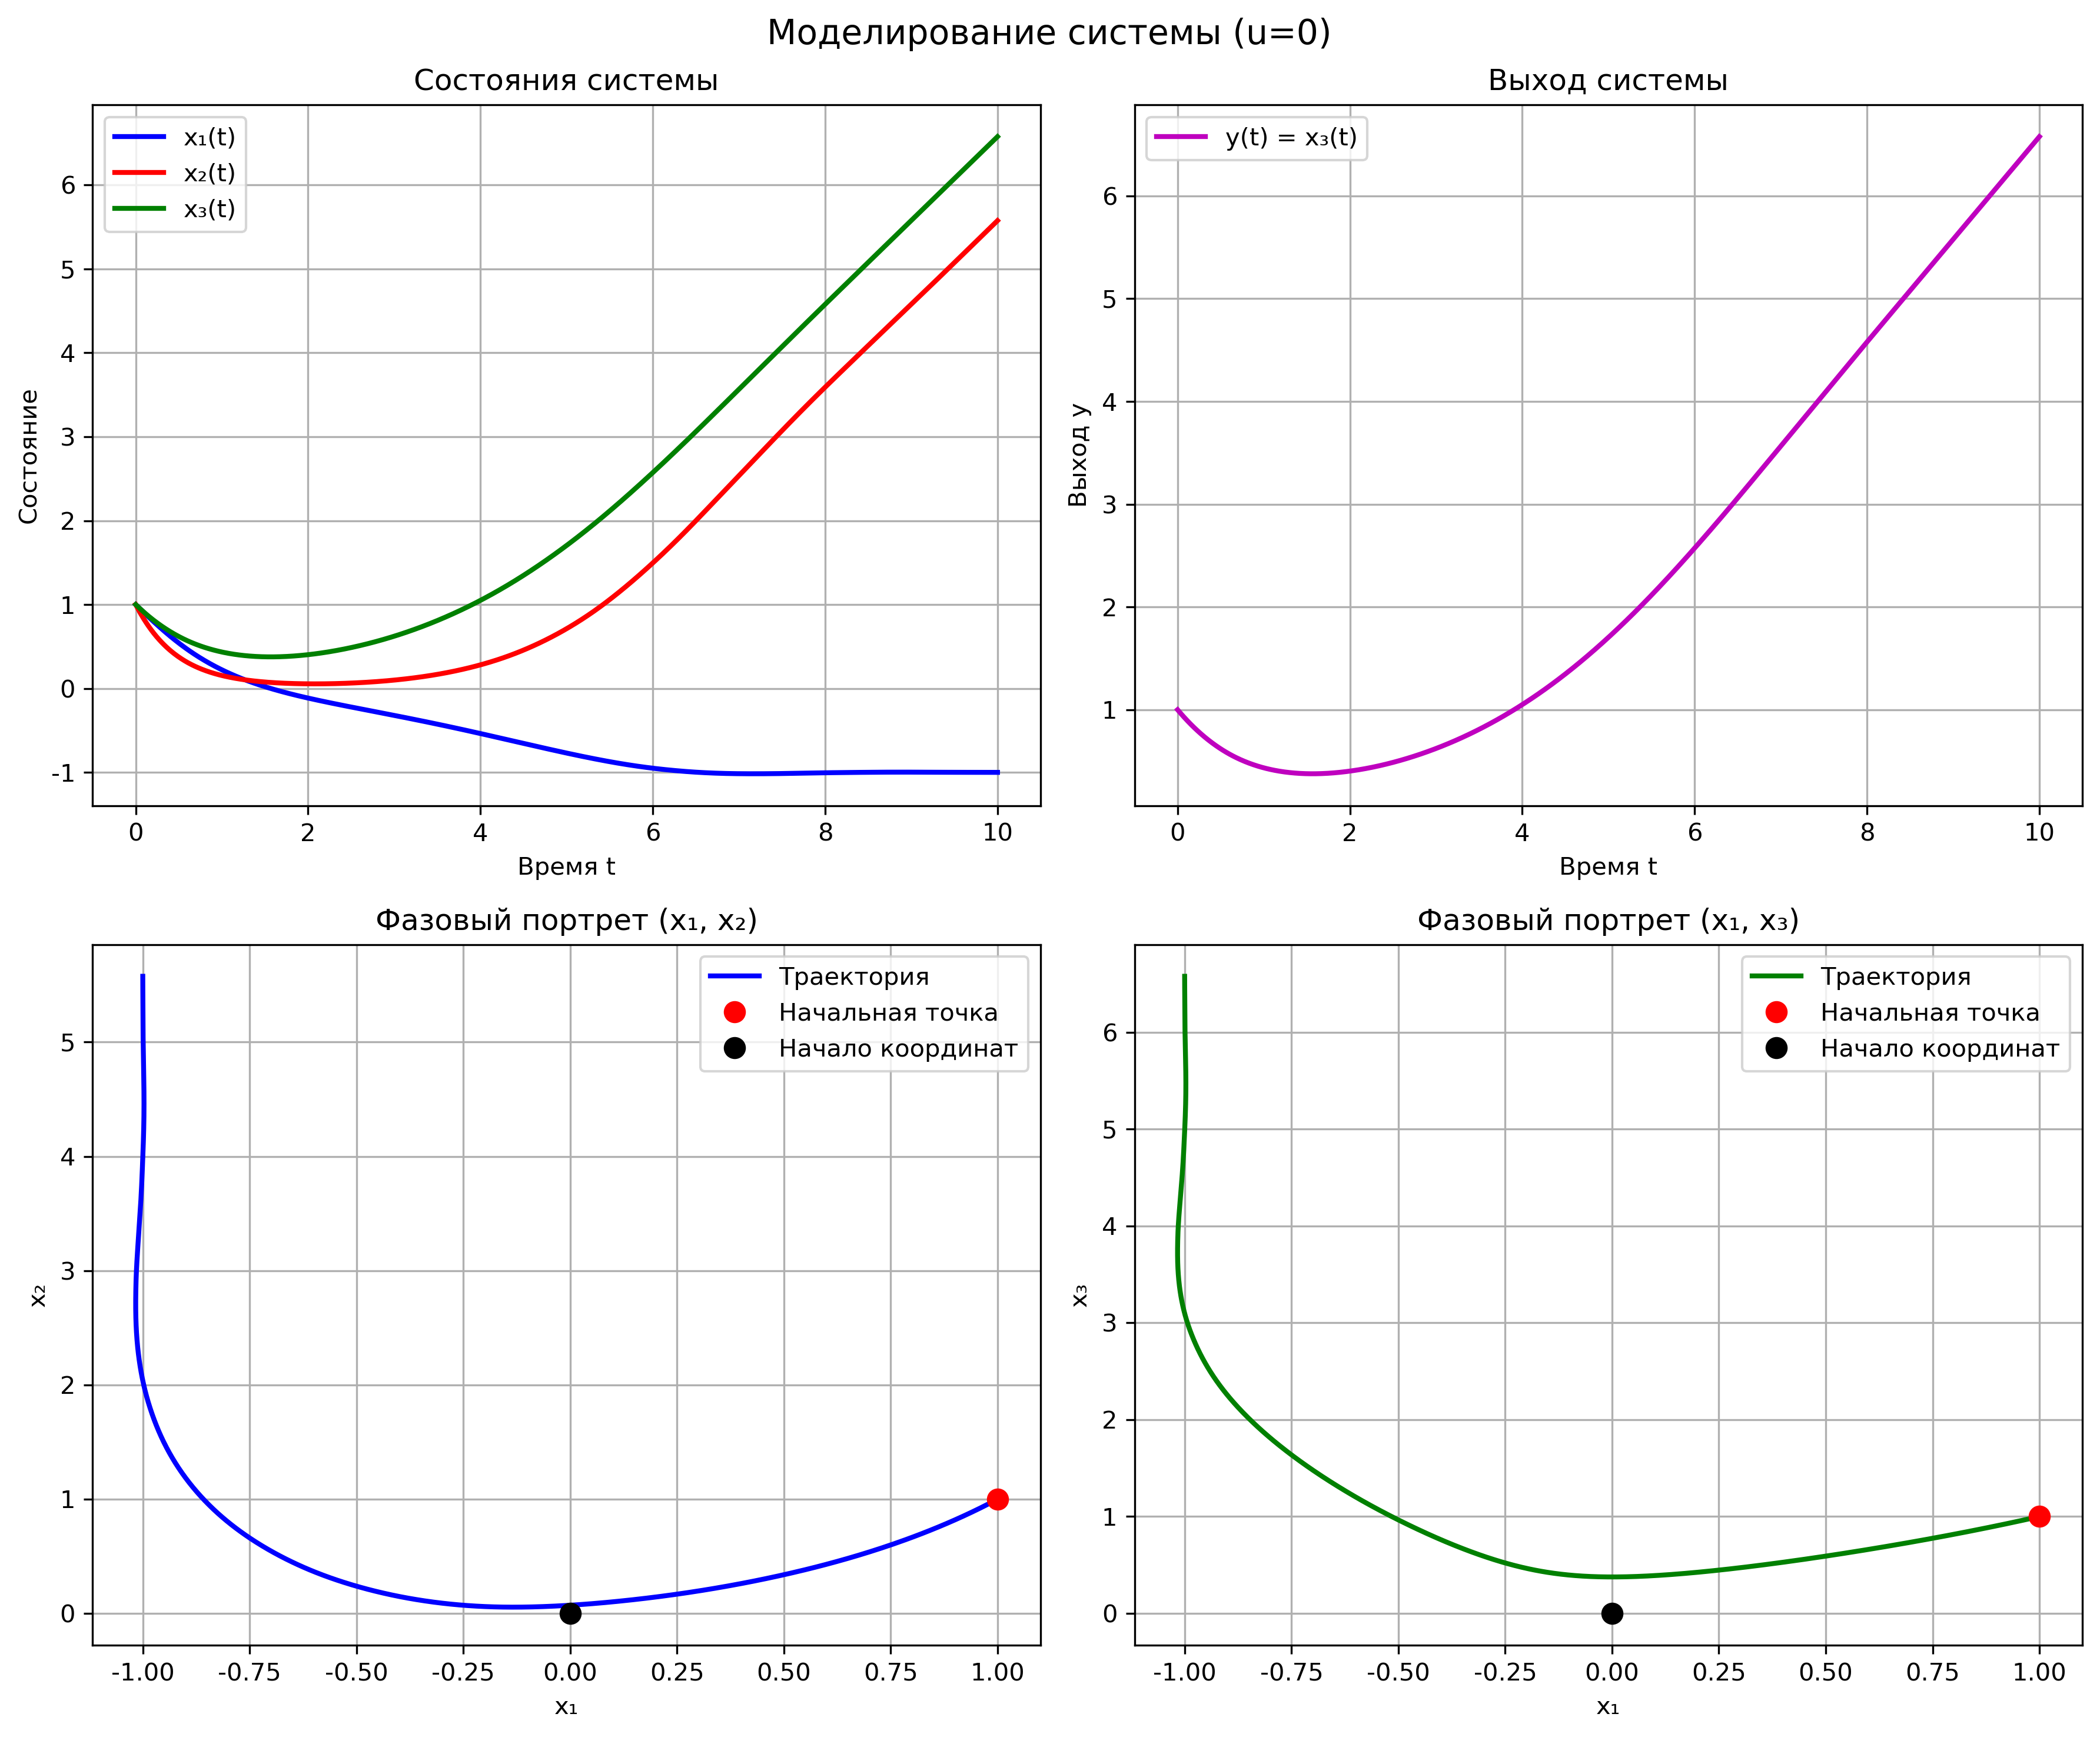
\includegraphics[width=0.9\textwidth]{task1/system_simulation.png}
\caption{Моделирование системы при нулевом управлении}
\label{fig:system_simulation}
\end{figure}

Результаты моделирования показывают поведение системы при нулевом управлении, демонстрируя внутреннюю динамику.

\subsection{Результаты задачи 1}

\textbf{Ответы:}
\begin{enumerate}
\item \textbf{Линеаризуемость:} Да, система линеаризуема по входу-выходу
\item \textbf{Относительная степень:} $r = 1$
\item \textbf{Нормальная форма:} получена с координатами $z_1 = x_3$, $z_2 = -x_1 + u$, $\eta_1 = x_1$, $\eta_2 = x_2$
\item \textbf{Область определения:} $\mathbb{R}^3$
\item \textbf{Минимально-фазовость:} Да, система минимально-фазовая
\end{enumerate}

\section{Задача 2. Синтез закона управления методом линеаризации обратной связью}

Рассмотрим систему:
\begin{align}
\dot{x}_1 &= -x_1 + x_2 \\
\dot{x}_2 &= x_1 - x_2 - x_1 x_3 + u \\
\dot{x}_3 &= x_1 + x_1 x_2 - 2x_3
\end{align}

Требуется найти закон управления с обратной связью по состоянию, обеспечивающий глобальную стабилизацию начала координат.

\subsection{Анализ управляемости}

Проверим управляемость системы через скобки Ли.

Векторное поле $g = [0, 1, 0]^T$ (коэффициенты при $u$).

Скобка Ли $[f, g] = \text{ad}_f g$:
\begin{align}
[f, g]_1 &= L_f g_1 - L_g f_1 = 0 - 0 = 0 \\
[f, g]_2 &= L_f g_2 - L_g f_2 = 0 - 1 = -1 \\
[f, g]_3 &= L_f g_3 - L_g f_3 = 0 - 0 = 0
\end{align}

Матрица управляемости в начале координат:
\begin{equation}
C = \begin{pmatrix} 0 & 0 & 0 \\ 1 & -1 & 0 \\ 0 & 0 & 0 \end{pmatrix}
\end{equation}

Ранг матрицы управляемости равен 2, что меньше размерности системы (3). Система не полностью управляема в начале координат.

\subsection{Проектирование регулятора}

Выберем выходную функцию $h(x) = x_1$ и применим метод линеаризации обратной связью.

\textbf{Шаг 1:} Вычисление производных Ли
\begin{align}
L_f h &= \frac{\partial h}{\partial x_1} f_1 + \frac{\partial h}{\partial x_2} f_2 + \frac{\partial h}{\partial x_3} f_3 \\
&= 1 \cdot (-x_1 + x_2) + 0 \cdot (x_1 - x_2 - x_1 x_3) + 0 \cdot (x_1 + x_1 x_2 - 2x_3) \\
&= -x_1 + x_2
\end{align}

\begin{align}
L_g L_f h &= \frac{\partial (L_f h)}{\partial x_1} g_1 + \frac{\partial (L_f h)}{\partial x_2} g_2 + \frac{\partial (L_f h)}{\partial x_3} g_3 \\
&= (-1) \cdot 0 + 1 \cdot 1 + 0 \cdot 0 = 1 \neq 0
\end{align}

Относительная степень $r = 2$.

\textbf{Шаг 2:} Синтез закона управления

Координаты нормальной формы:
\begin{align}
z_1 &= h = x_1 \\
z_2 &= L_f h = -x_1 + x_2
\end{align}

Вычисляем $L_f^2 h$:
\begin{align}
L_f^2 h &= \frac{\partial (L_f h)}{\partial x_1} f_1 + \frac{\partial (L_f h)}{\partial x_2} f_2 + \frac{\partial (L_f h)}{\partial x_3} f_3 \\
&= (-1) \cdot (-x_1 + x_2) + 1 \cdot (x_1 - x_2 - x_1 x_3) + 0 \cdot (x_1 + x_1 x_2 - 2x_3) \\
&= x_1 - x_2 + x_1 - x_2 - x_1 x_3 = 2x_1 - 2x_2 - x_1 x_3
\end{align}

Закон управления:
\begin{equation}
u = \frac{v - L_f^2 h}{L_g L_f h} = \frac{v - (2x_1 - 2x_2 - x_1 x_3)}{1} = v - 2x_1 + 2x_2 + x_1 x_3
\end{equation}

Выбираем $v = -k_1 z_1 - k_2 z_2 = -k_1 x_1 - k_2 (-x_1 + x_2)$ для стабилизации.

При $k_1 = 2$, $k_2 = 3$:
\begin{equation}
u = -2x_1 - 3(-x_1 + x_2) - 2x_1 + 2x_2 + x_1 x_3 = -x_1 - x_2 + x_1 x_3
\end{equation}

\subsection{Моделирование управляемой системы}

\begin{figure}[H]
\centering
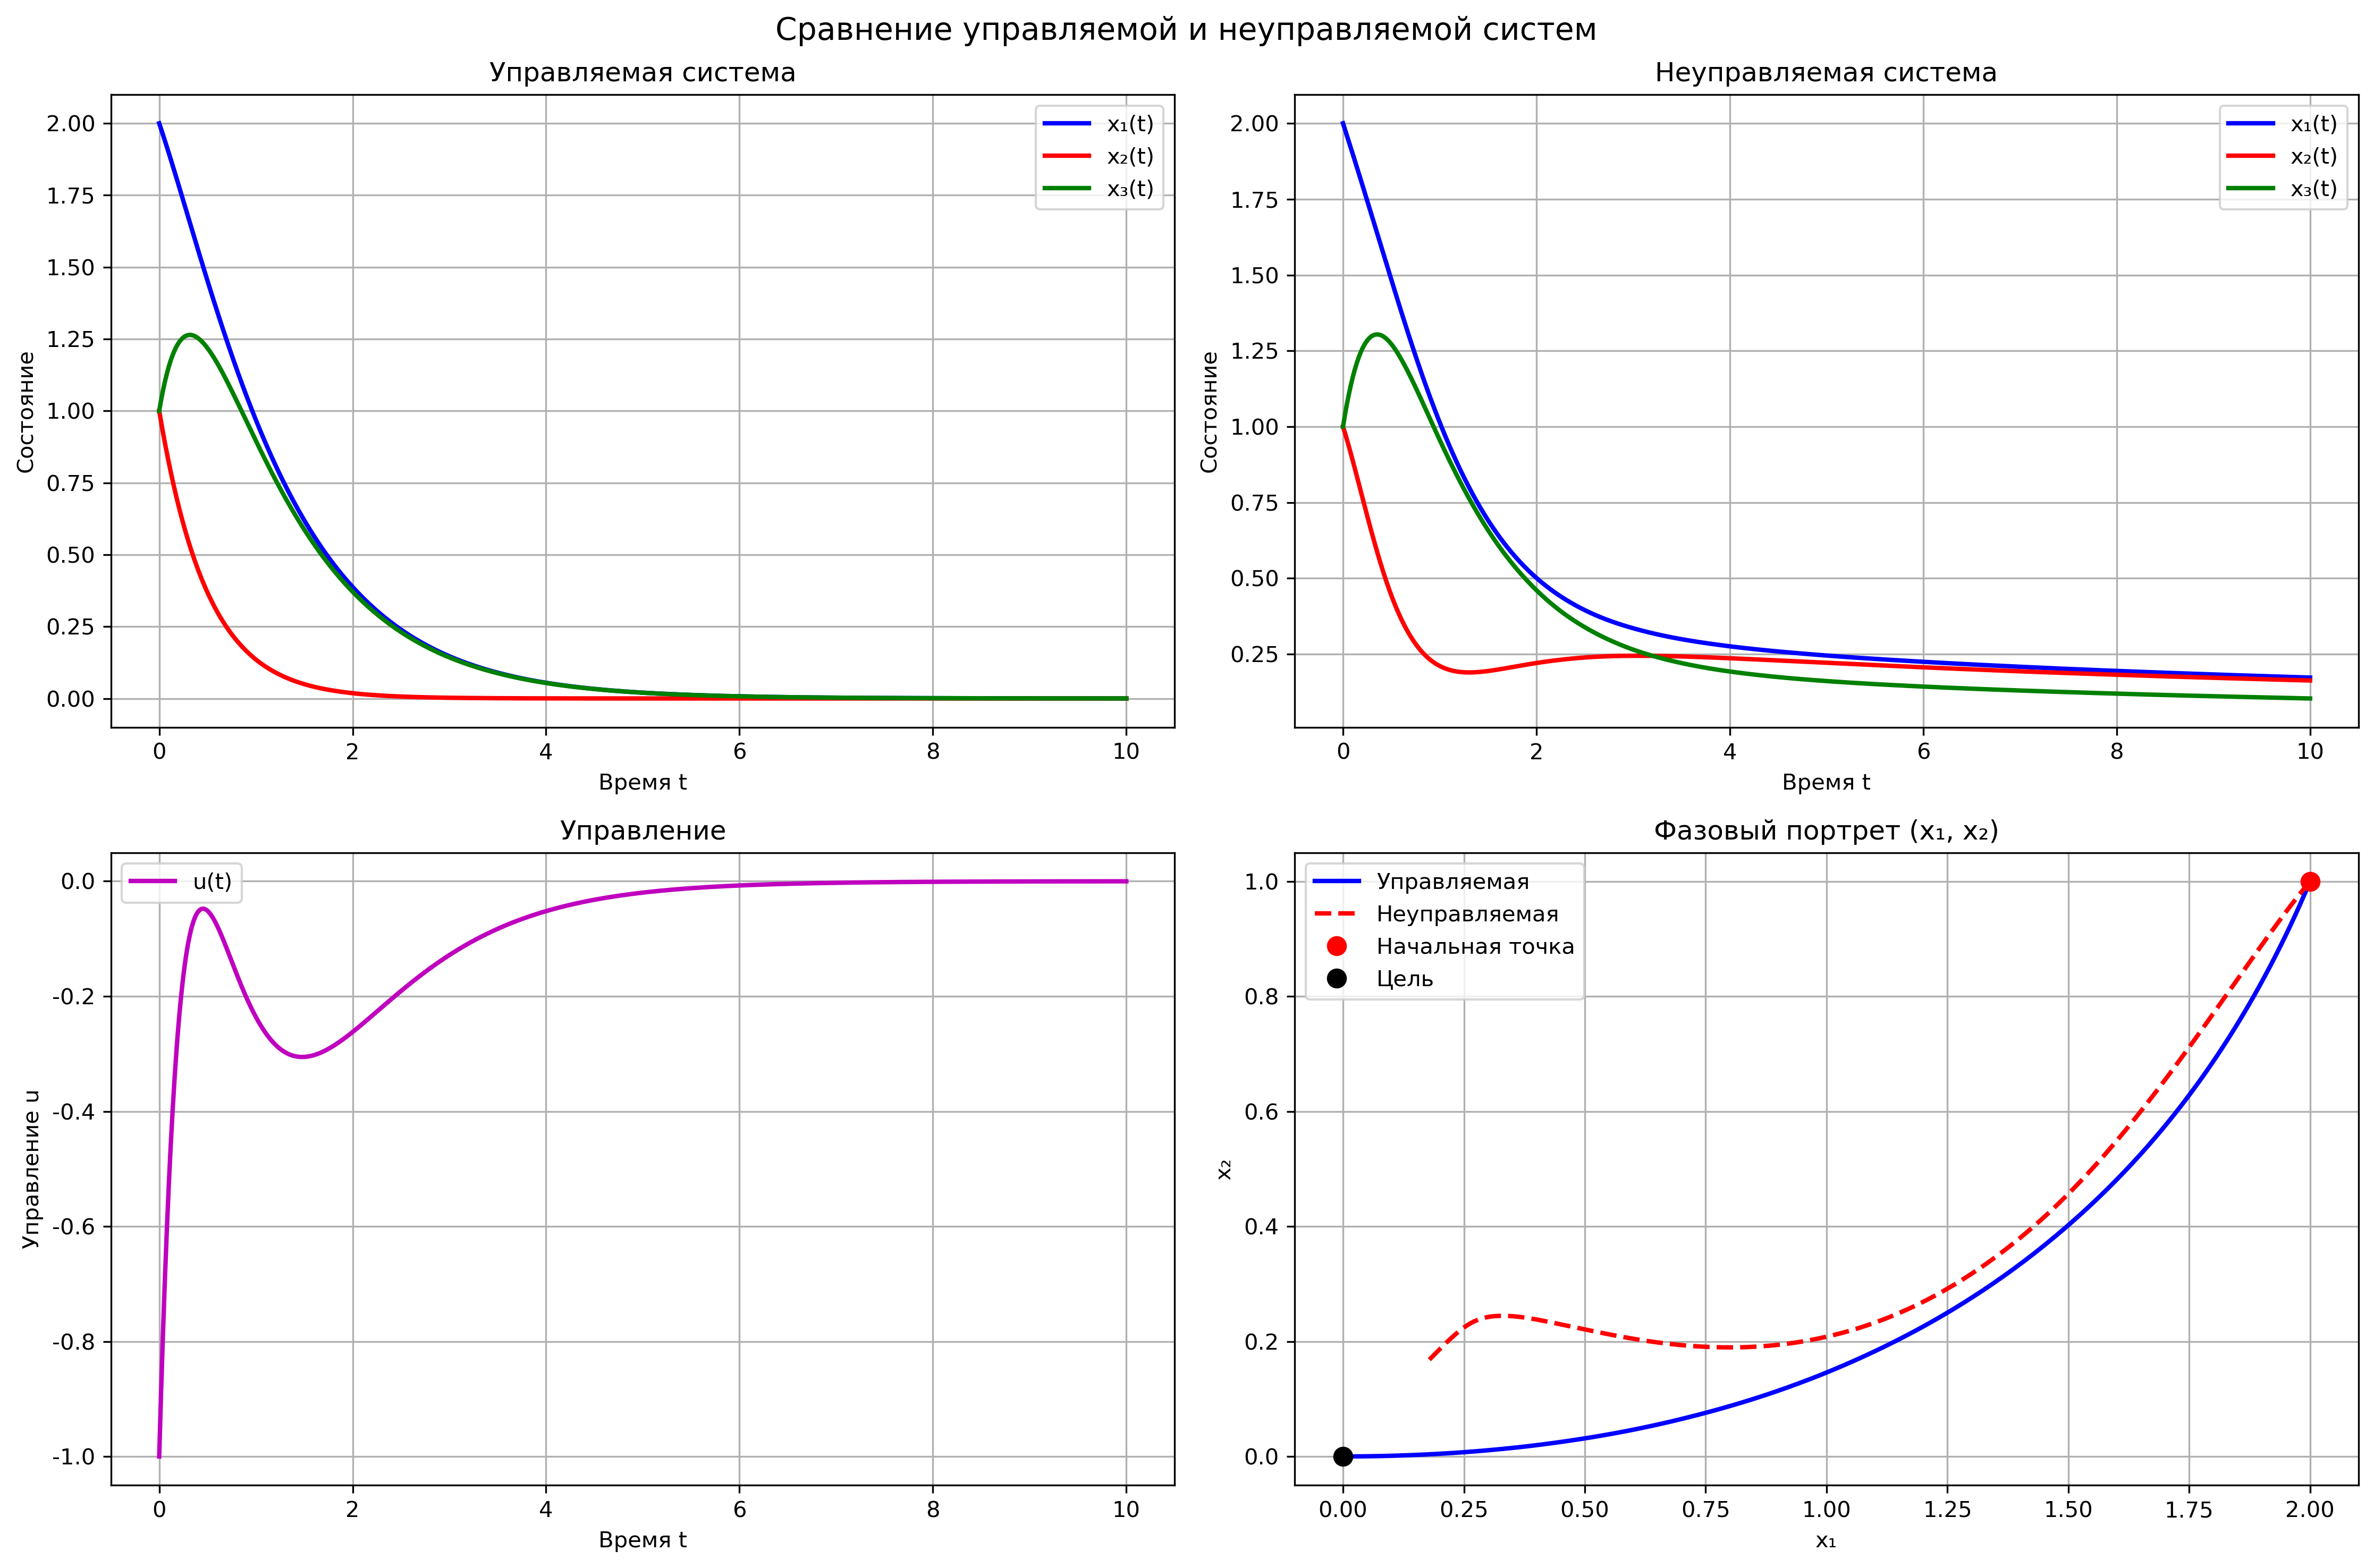
\includegraphics[width=0.9\textwidth]{task2/feedback_linearization.png}
\caption{Сравнение управляемой и неуправляемой систем}
\label{fig:feedback_linearization}
\end{figure}

Результаты моделирования показывают:
\begin{itemize}
\item Управляемая система экспоненциально сходится к началу координат
\item Неуправляемая система остается неустойчивой
\item Закон управления обеспечивает глобальную стабилизацию
\end{itemize}

\subsection{Результаты задачи 2}

\textbf{Закон управления:} $u = -x_1 - x_2 + x_1 x_3$

\textbf{Относительная степень:} $r = 2$

\textbf{Стабилизация:} Глобальная стабилизация начала координат достигнута

\section{Заключение}

В данной лабораторной работе были рассмотрены методы линеаризации обратной связью для нелинейных систем управления. Выполнены следующие задачи:

\begin{enumerate}
\item \textbf{Анализ линеаризуемости по входу-выходу:} для первой системы установлена линеаризуемость с относительной степенью $r = 1$ и минимально-фазовость.

\item \textbf{Преобразование в нормальную форму:} получены координаты нормальной формы с областью определения $\mathbb{R}^3$.

\item \textbf{Синтез закона управления:} для второй системы синтезирован закон управления $u = -x_1 - x_2 + x_1 x_3$, обеспечивающий глобальную стабилизацию начала координат.

\item \textbf{Численное моделирование:} подтверждена эффективность синтезированных законов управления.
\end{enumerate}

Работа продемонстрировала эффективность применения методов линеаризации обратной связью к практическим задачам управления нелинейными системами. Все поставленные задачи решены с использованием численного моделирования и визуализации результатов.
                                     % Основной текст отчета

\printbibliography[title=Список использованных источников] % Автособираемый список литературы

\end{document}
